\documentclass{beamer}

\usetheme{Madrid}
\usecolortheme{beaver}

\usepackage{amsmath}
\usepackage{amssymb}
\usepackage{graphicx}
\usepackage{subcaption}
\usepackage{bbm}
\usepackage{booktabs}
\usepackage{url}
\usepackage{cancel}

\usepackage[style=authoryear]{biblatex}
\addbibresource{references.bib}

\renewcommand{\footnotesize}{\tiny}

\title[Power law attention biases]{Power law attention biases for molecular transformers}
\author{Jay Shen}

\begin{document}

% -------------------------------------------------------
\begin{frame}
    \titlepage
\end{frame}

% =======================================================
\section{Motivation}
% =======================================================

\begin{frame}{Why predict molecular properties?}

Properties like energies, forces, and orbital levels drive drug discovery, catalysis, and materials design.

\vspace{1em}

The gold standard---density functional theory (DFT)---is accurate but expensive: minutes to hours per molecule, scaling poorly with system size.

\vspace{1em}

\textbf{Goal:} train a neural network on DFT-labeled data, then run inference in milliseconds. 

\end{frame}

% -------------------------------------------------------
\begin{frame}{What does the data look like?}

A molecule is a 3D point cloud:
\begin{itemize}
    \item Atomic numbers $z_i \in \mathbb{N}$
    \item 3D coordinates $\mathbf{r}_i \in \mathbb{R}^3$
\end{itemize}

\vspace{1em}

Scalar targets (e.g.\ total energy) must be invariant under:
\begin{itemize}
    \item Translations and rotations of the whole molecule
    \item Permutations of atom indices
\end{itemize}

\vspace{1em}

No canonical ordering, no grid, no absolute coordinates---just relative geometry.

\end{frame}

% =======================================================
\section{Background}
% =======================================================

\begin{frame}{The molecular ML landscape}

Equivariant graph neural networks dominate molecular property prediction\footcite{li-mlip-review}\footcite{jacobs-mlip-review}.

\vspace{1em}

Transformers, despite ruling vision and language, are rarely competitive here. Why the asymmetry?

\vspace{1em}

\textbf{Hypothesis:} transformers lack good \textit{inductive biases} for many-body geometry.

\end{frame}

% -------------------------------------------------------
\begin{frame}{The problem with dot-product attention}

The root of the problem lies in the attention mechanism:
\[
A_{ij}=\mathrm{softmax}_j\left( \frac{\mathbf{q}_i \mathbf{k}_j^T}{\sqrt{d_k}} \right)
\]

This form implies the token embedding must encode \textit{both} the token's identity \textit{and} its relationships to other tokens. 
\vspace{1em}

\begin{itemize}
    \item[$\rightarrow$] Fine for language/images, absolute token indices $\implies$ positional encodings
    \item[$\rightarrow$] Bad for point clouds: no natural indices and structure is continuous.
\end{itemize}

\end{frame}

% -------------------------------------------------------
\begin{frame}{Attention biases}

Consider adding a pairwise term $b_{ij}$ inside the softmax:
\[
A_{ij}=\mathrm{softmax}_j\left( \frac{\mathbf{q}_i \mathbf{k}_j^T}{\sqrt{d_k}} + b_{ij} \right)
\]

\begin{itemize}
    \item Permutation invariance for free. 
    \item Naturally \textit{pairwise}, just like all physical interactions.
    \item \textbf{Easy to construct given a notion of distance between tokens.}
\end{itemize}

% \vspace{1em}

% Similar techniques have been used elsewhere (vision transformers on image grids, distance-kernel biases on molecules).

\end{frame}

% =======================================================
\section{Power Law Attention Biases}
% =======================================================

\begin{frame}{Power law attention biases}

Consider the $E(3)$-equivariant bias $b_{ij}=p \log ||\mathbf{r}_i - \mathbf{r}_j||$.

\vspace{1em}

Through the softmax:
\begin{equation*}
\begin{split}
    A_{ij} &= \text{softmax}_j \biggr [\frac{\mathbf{q}_{i} \mathbf{k}_j^T}{\sqrt{d_k}} + p \log || \mathbf{r}_i - \mathbf{r}_j || \biggr] \\
    &\propto || \mathbf{r}_i - \mathbf{r}_j ||^{p}\exp \biggr[ \frac{\mathbf{q}_{i} \mathbf{k}_j^T}{\sqrt{d_k}} \biggr]
\end{split}
\end{equation*}

The bias \textit{weights} attention by a power of the interatomic distance.

\vspace{1em}

\textbf{Analogous to Coulomb's law:} interaction strength is set by both charges (embeddings) and distance.

\end{frame}

% -------------------------------------------------------
\begin{frame}{Design choices for $p$}

The remaining degrees of freedom lie in $p$. Several options:
\begin{itemize}
    \item Fix $p = -1$ (echoes potential-energy fall-off).
    \item Learn $p \in \mathbb{R}$.
    \item Learn $p \in \mathbb{R}_-$ via reparameterization $p = -e^\theta$.
\end{itemize}

\vspace{1em}

\textbf{Edge case:} singularity when $i = j$. Resolve by masking out the diagonal.

\end{frame}

% =======================================================
\section{Experiments}
% =======================================================

\begin{frame}{Setup}

Standardized transformer architecture across all baselines:
\begin{table}
    \scriptsize
    \centering
    \begin{tabular}{lc}
    \toprule
    Embedding dimension & 128 \\
    Number of layers & 8 \\
    Number of attention heads & 8 \\
    Dropout & 0.1 \\
    Number of epochs & 128 \\
    Batch size & 64 \\
    Learning rate & 0.0001 \\
    Weight Decay & 0.00001 \\
    \bottomrule
    \end{tabular}
\end{table}

Roughly 1.5M parameters per model, trains in 1 hour on 1 V100 GPU.

\end{frame}

% -------------------------------------------------------
\begin{frame}{Benchmarks}

We train and evaluate on two DFT datasets:
\begin{itemize}
    \item \textbf{QM9}: 134k molecules (~5M tokens) labeled with orbital energies HOMO, LUMO and state energies $U$, $H$, $G$.
    \item \textbf{SPICE}: 1.1M molecules (~50M tokens) labeled with formation energy $U_F$.
\end{itemize}

\end{frame}

% -------------------------------------------------------
\begin{frame}{Results}
\begin{table}[ht]
    \scriptsize
    \centering
    \begin{tabular}{l c ccccc c c}
        \toprule
        &&\multicolumn{5}{c}{QM9} && \multicolumn{1}{c}{SPICE} \\
        \cline{3-7}\cline{9-9}
        \noalign{\vskip 2pt}
        Structural bias && HOMO & LUMO & $U$ & $H$ & $G$ && $U_F$\\
        \hline
        \noalign{\vskip 2pt}
        Transformer && 0.34 & 0.74 & 24 & 24 & 24 && 10 \\
        Graph Attention && 0.12 & 0.14 & 29 & 29 & 30 && - \\
        RWPE && 0.14 & 0.20 & 42 & 42 & 42 && - \\
        \noalign{\vskip 2pt}
        Attention bias && & & & & && \\
        \cline{0-0}
        \noalign{\vskip 2pt}
        Gaussian kernel && 0.08 & 0.10 & 21 & 21 & 21 && - \\
        Power law $p=-1$ && 0.11 & 0.13 & 26 & 26 & 26 && 7 \\
        Power law $p \in \mathbb{R}$ && 0.12 & 0.14 & 25 & 25 & 25 && 5 \\
        Power law $p\in \mathbb{R}_-$ && 0.11 & 0.12 & 21 & 21 & 21 && 5 \\
        \bottomrule
    \end{tabular}
    \caption{Test ensemble MAE (eV).}
\end{table}

Attention biases beat positional encodings and graph attention, while matching Gaussian kernels at a fraction of the parameters.

\end{frame}

% -------------------------------------------------------
\begin{frame}{Learned exponents}
\begin{figure}[ht]
    \centering
    \begin{subfigure}[t]{0.25\textwidth}
        \centering
        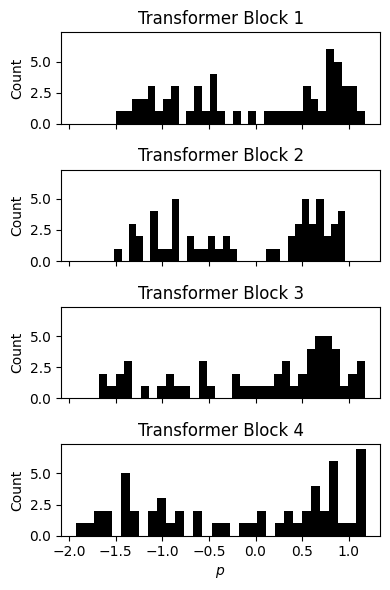
\includegraphics[width=\linewidth]{figures/exponents_unconstrained.png}
        \caption{$p\in\mathbb{R}$}
    \end{subfigure}%
    \hspace{2.5em}
    \begin{subfigure}[t]{0.25\textwidth}
        \centering
        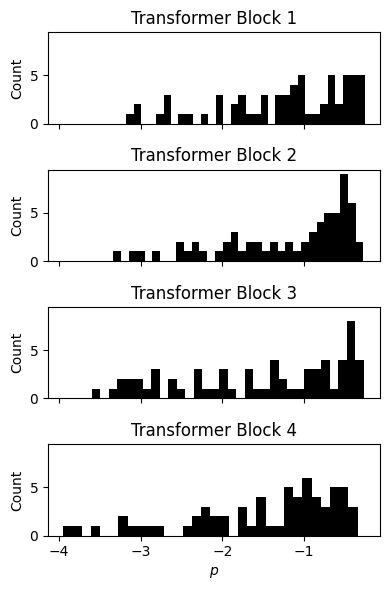
\includegraphics[width=\linewidth]{figures/exponents_negative.png}
        \caption{$p\in\mathbb{R}^-$}
    \end{subfigure}
    \caption{Histograms of learned exponents over 7-model ensembles.}
\end{figure}

Exponents don't tend to any specific power law and when unconstrained even drift positive (unphysical). 

\end{frame}

% =======================================================
\section{Ablation Study}
% =======================================================

\begin{frame}{Ablating dot-product attention}

How much modeling power do power law attention biases have? Test by ablating the dot-product:

\[
A_{ij}=\mathrm{softmax}_j\left(\: \cancel{\frac{\mathbf{q}_i \mathbf{k}_j^T}{\sqrt{d_k}}}  + b_{ij} \right) \quad \rightarrow \quad A_{ij} = \mathrm{softmax}_j(b_{ij})
\]

This form is basically weighted message passing on a complete graph, and structure is fully decoupled from token content.

\vspace{1em}

\textbf{Bonus: } no dot products $\implies$ cheaper to evaluate.  

\end{frame}

% -------------------------------------------------------
\begin{frame}{Effect of ablation}
\begin{table}[ht]
    \scriptsize
    \centering
    \begin{tabular}{l c ccccc}
        \toprule
         && HOMO & LUMO & $U$ & $H$ & $G$ \\
        \hline
        \noalign{\vskip 2pt}
        Transformer && 0.34 & 0.74 & 24 & 24 & 24 \\
        \noalign{\vskip 2pt}
        Attention bias &&&&&& \\
        \cline{0-0}
        \noalign{\vskip 2pt}
        Gaussian kernel && 0.1 (+8\%) & 0.1 (+7\%) & 20 (-5\%) & 20 (-6\%) & 20 (-7\%) \\
        Power law $p=-1$ && 0.1 (+14\%) & 0.2 (+19\%) & 27 (+3\%) & 27 (+2\%) & 27 (+4\%) \\
        Power law $p\in \mathbb{R}$ && 0.1 (+9\%) & 0.1 (+11\%) & 26 (+3\%) & 25 (+2\%) & 25 (+3\%) \\
        Power law $p \in \mathbb{R}_-$ && 0.1 (+11\%) & 0.1 (+12\%) & 25 (+9\%) & 25 (+8\%) & 25 (+9\%) \\
        \bottomrule
    \end{tabular}
    \caption{Ensemble MAE (eV); percent change from unablated in parentheses.}
\end{table}

\begin{itemize}
    \item Loss increases modestly---and ablated models still beat the vanilla transformer.
    \item Gaussian kernel biases actually \textit{improve} on $U$, $H$, $G$ when the dot-product is removed.
\end{itemize}

\end{frame}

% =======================================================
\section{Conclusions}
% =======================================================

\begin{frame}{Takeaways}

Power law attention biases are:
\begin{itemize}
    \item Simple and physically motivated.
    \item More effective than most other inductive biases. 
    \item Only matched by Gaussian kernels, which are much more expensive. 
    \item Highly effective on their own, as shown by ablation. 
\end{itemize}

\textbf{Caveat:} Uninterpretable learned exponents $\implies$ physicality of the mechanism is dubious. 

\end{frame}

% -------------------------------------------------------
\begin{frame}{Questions/Limitations}

\begin{itemize}
    \item How do these results change with scale? 
    \item How do these results change out-of-distribution? 
    \item How accurate and useful are first derivatives (forces)?
    \item Are predictions stable in dynamical settings?
    \item How do initializations affect learned $p$?
    \item Are models inhibited by gradient flow issues in $p$?
    \item Can message passing layers cheapen large models? 
\end{itemize}

\end{frame}

% -------------------------------------------------------
\begin{frame}
\centering
End
\end{frame}

\end{document}
